\section{Practical - ADC on the Pi}
Prac 5 is going to serve as an introduction to the mini-project, requiring you to configure some basic systems before integrating them all into the final device. Part of the deliverables for this prac is a short demo video which you could record on a smartphone and upload as part of the assignment, see Section \ref{prac4sub}.

In this prac you're going to sample temperature data from the ADC every 10 seconds. We're going to be using the \href{https://learn.adafruit.com/mcp3008-spi-adc/python-circuitpython}{Adafruit MCP3008 Library for Python}.

\subsection{Circuit}
You need to connect the following:
\begin{itemize}
    \item MCP3008 CLK to Pi SCLK
    \item MCP3008 DOUT to Pi MISO
    \item MCP3008 DIN to Pi MOSI
    \item MCP3008 CS/SHDN to Pi CE0
    \item MCP3008 VDD to Pi 3.3V
    \item MCP3008 VREF to Pi 3.3V
    \item MCP3008 AGND to Pi GND
    \item MCP3008 DGND to Pi GND
    \item Read the \href{http://ww1.microchip.com/downloads/en/DeviceDoc/20001942G.pdf}{data sheet for the MCP9700} and connect it correctly to channel 1 (pin 2) of the ADC.
    \item Add a button on a suitable GPIO pin
\end{itemize}

\begin{figure}[H]
\centering
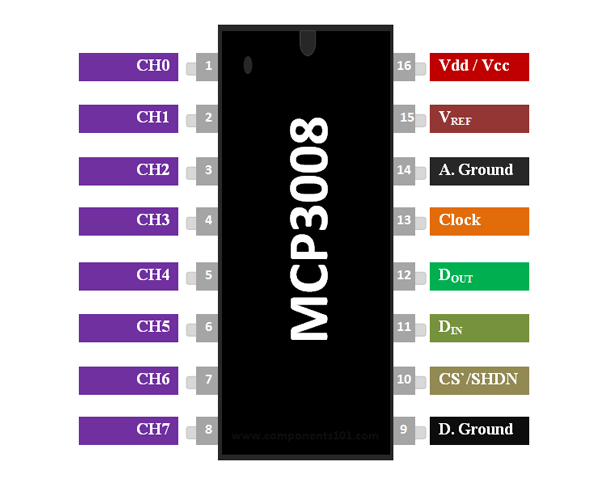
\includegraphics[width=0.6\columnwidth]{Figures/MCP3008Pinout}
\caption{The pinout of the MCP3008}
% \label{}
\end{figure}

\subsection{Walkthrough}
\begin{enumerate}
    \item Enable SPI using the raspi-config tool
    \item Install the MCP3008 Adafruit library
    \begin{lstlisting}[gobble=4]
    $ sudo apt-get update
    $ sudo apt install build-essential python3-dev python3-smbus python3-pip
    $ sudo pip3 install adafruit-circuitpython-mcp3xxx
    \end{lstlisting}
    \item Build the circuit described above.
    \item Create a new python file
    \item Place the following code in it:
    \begin{lstlisting} [gobble=4]
    import busio
    import digitalio
    import board
    import adafruit_mcp3xxx.mcp3008 as MCP
    from adafruit_mcp3xxx.analog_in import AnalogIn

    # create the spi bus
    spi = busio.SPI(clock=board.SCK, MISO=board.MISO, MOSI=board.MOSI)

    # create the cs (chip select)
    cs = digitalio.DigitalInOut(board.D5)

    # create the mcp object
    mcp = MCP.MCP3008(spi, cs)

    # create an analog input channel on pin 0
    chan = AnalogIn(mcp, MCP.P0)

    print('Raw ADC Value: ', chan.value)
    print('ADC Voltage: ' + str(chan.voltage) + 'V')
    \end{lstlisting}
    If you run this code you will see the reading from the LDR. Cover the sensor and run the code again. The reading should change.
    \item Adapt your code to read from both sensors and print to terminal every ten seconds. You \textbf{must} use a thread. You can read about simple threading in Python \href{http://wiki.ee.uct.ac.za/RaspberryPi:ProgrammingInPython}{here}. The output of your application should look as follows:
    \begin{lstlisting}[gobble=4]
    Runtime     Temp Reading    Temp	
    0s          <ADC value>	    <converted temp>  C
    10s         <ADC value>	    <converted temp>  C
    20s         <ADC value>	    <converted temp>  C
    30s         <ADC value>	    <converted temp>  C
    40s         <ADC value>	    <converted temp>  C
    50s         <ADC value>	    <converted temp>  C
    60s         <ADC value>	    <converted temp>  C
    \end{lstlisting}
    \item Runtime must be calculated, and not be implemented as a counter
    \item Add a button to toggle the rate of sampling between 10s, 5s and 1s
\end{enumerate}

\subsection{Requirements for submission}
\label{prac4sub}
There are two items you need to uploaded to Vula for submission of this practical assignment: 
\begin{enumerate}
    \item Your prac report provided as a single PDF file, named \verb|Prac5_<studnum1>_<studnum2>.pdf|
    \item A short demo video in which you present your design and implementation (see demo marking guide in Table \ref{tbl:Prac5DemoValidation} below).
\end{enumerate}


\textbf{Report Requirements}

The report should contain the following:
\begin{enumerate}
    \item The circuit diagram you used
    \item A paragraph on your validation and testing for the values you got from the ADC for both light and temperature
    \item Your Python code (screenshots of code will not be marked)
\end{enumerate}
Marks will be awarded for:
\begin{itemize}
    \item Neatness (circuit diagram and code)
    \item Correctness
    \item Using threads correctly
    \item Correct implementation of the temperature reading algorithm
\end{itemize}

\textbf{Demo Marking Guide}

Marks will be deducted for:
\begin{itemize}
    \item Not following instructions
    \item Plagiarism/Copying
\end{itemize}

You can prepare a short video, about 5 minutes will probably be sufficient. There is no minimum duration, but you need to respond to the aspects as listed in the marksheet below; but we do \textit{not} want videos beyond 10 minutes in length. The demo should respond to the following aspects (the marking allocations are shown on the right):

\label{sec:ProjAValidation}
\begin{table}[H]
\caption{The Mark sheet for the demo aspect of Prac5}
\label{tbl:Prac5DemoValidation}
\centering
\resizebox{\textwidth}{!}{%
\begin{tabular}{|l|l|l|r|c|}
\hline
% \multicolumn{3}{|l|}{{\ul \textbf{Project Validation Sheet}}}  & \multicolumn{2}{l|}{\begin{tabular}[c]{@{}l@{}}\textbf{Marked by:} \\ \\\end{tabular}} \\ \hline
% \multicolumn{7}{|l|}{\begin{tabular}[c]{@{}l@{}}\textbf{Student Numbers:} \\ \\ \\\end{tabular}} \\ \hline
\textbf{Category} & \textbf{Item} & \textbf{Description} & \multicolumn{1}{c|}{Max Mark} & \begin{tabular}[c]{@{}c@{}}Attempt\\ 1\end{tabular} \\ \hline 

\textbf{Intro} & \begin{tabular}[c]{@{}l@{}}Intro \\ and division of \\ workload \end{tabular} & \begin{tabular}[c]{@{}l@{}}Start off the demo by\\ indicating your prac team \\ members. \\ Indicate how you \\ divided up the work \end{tabular} & 6 &    \\ \hline

\textbf{Design} & Design and connections & \begin{tabular}[c]{@{}l@{}}Indicate the way\\ you hooked up the ADC \\ (using a circuit diagram or alternate \\ clear visualization) \\ and present the software design \\ e.g block diagram or flow chart \\ of your program \end{tabular} & 5 &  \\ \hline
 &  & \begin{tabular}[c]{@{}l@{}}Point to significant parts of \\ your code that \\ concerns the hardware and \\ any timing aspects \\ (use of comments,\\ and reminders in the \\ code, e.g. of things to draw \\ attention to in the demo are recommended)\end{tabular} & 5 &  \\ \hline
 
ADC Test & Testing Implementation & \begin{tabular}[c]{@{}l@{}}Run through the \\ operation of your \\ prototype  (e.g. increase light \\ decrease light, etc) \end{tabular} & 10 &  \\ \hline

%  & Potentiometer & \begin{tabular}[c]{@{}l@{}}Responds to changes input, \\ reading displayed is between\\ 0 and 3.3V\end{tabular} & 2 &  &  &  \\ \hline
Conclude & Conclude the presentation & \begin{tabular}[c]{@{}l@{}}Report on the extent the test was \\ successful provide some suggestions \\ for how you might improve \\ things or add features if time allowed \end{tabular} & 4 & \begin{tabular}[c]{@{}l@{}} \end{tabular}  \\ \hline
Mark &  &  & 30 & \begin{tabular}[c]{@{}l@{}} \\ \\\end{tabular} \\ \hline
\end{tabular}%
}
\end{table}

